\documentclass[border=10pt]{standalone}
\usepackage[svgnames]{xcolor}
\usepackage{amsmath}
\usepackage{pgfplots}
\pgfplotsset{compat=newest}
\usepackage[sfdefault]{FiraSans}
\usepackage{FiraMono}
\renewcommand*\familydefault{\sfdefault}
\begin{document}
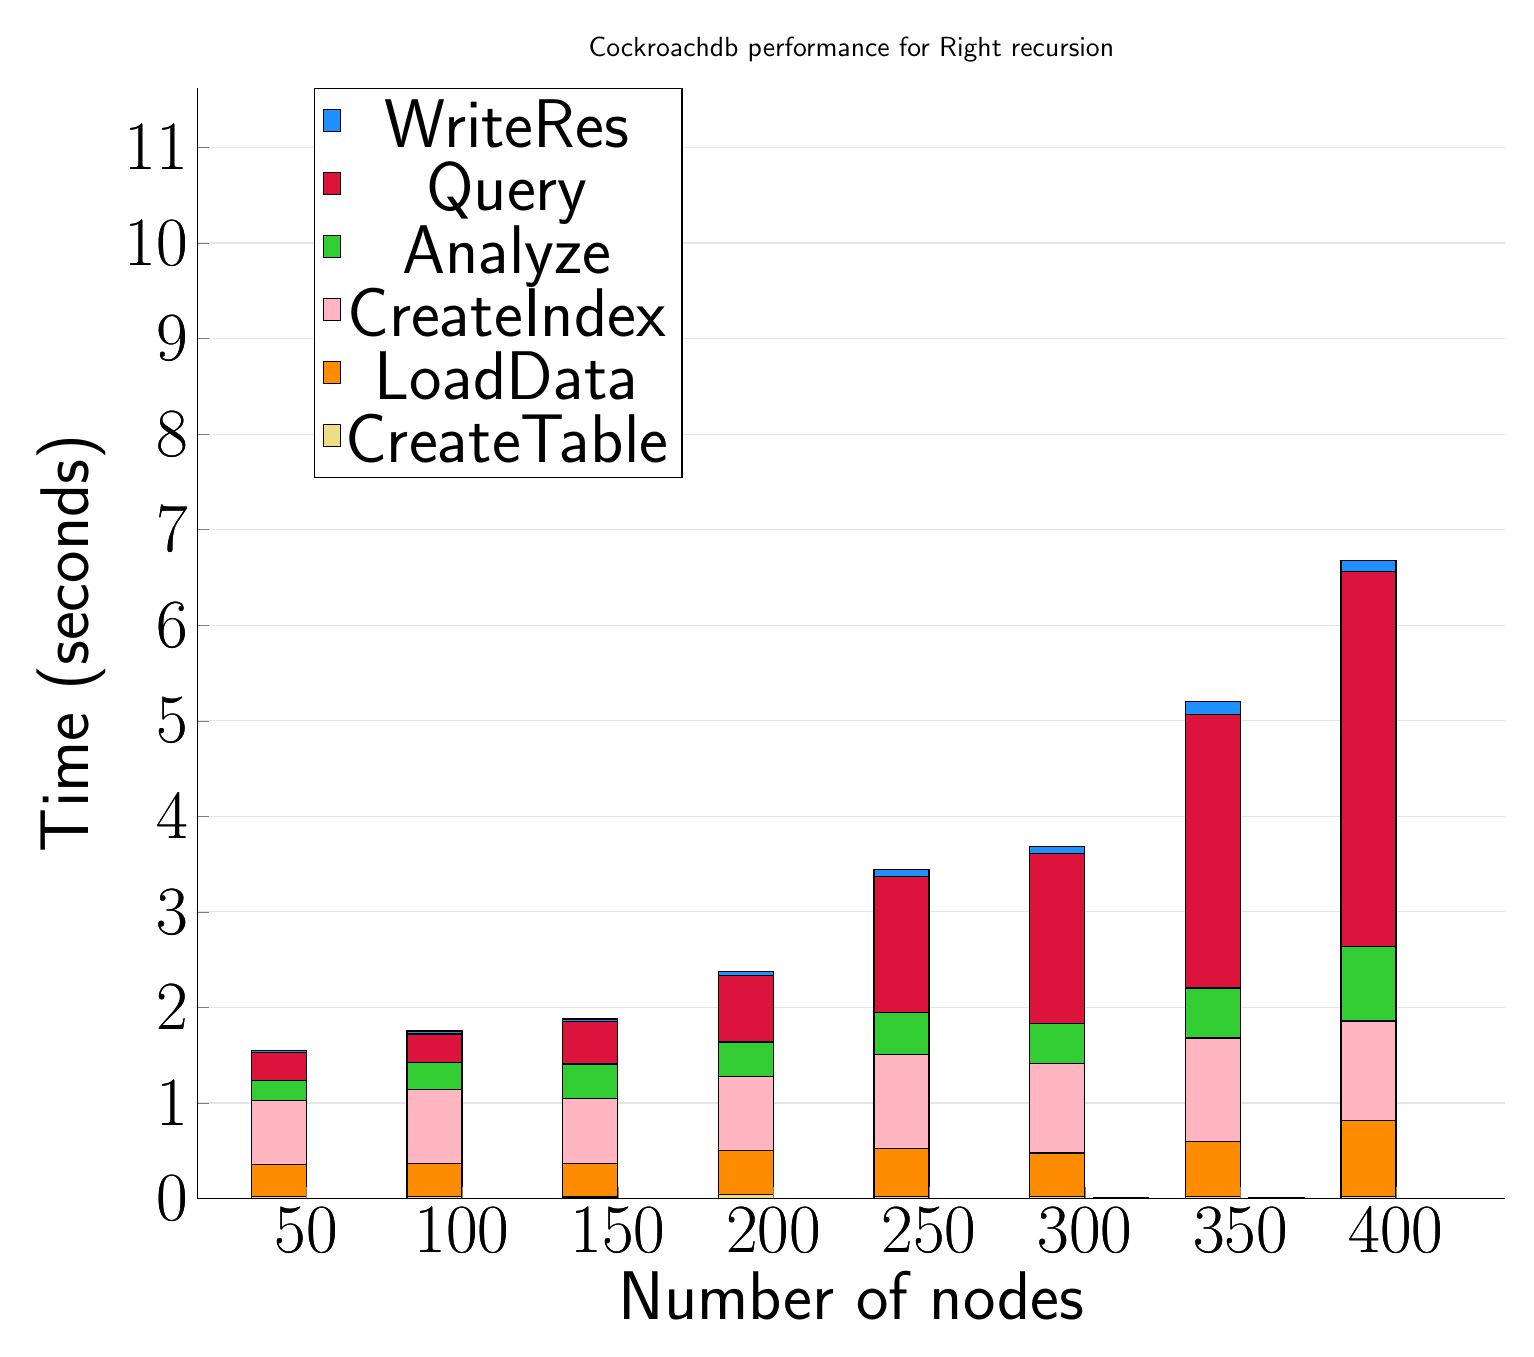
\begin{tikzpicture}
\begin{axis}[
   ybar stacked,
   title={Cockroachdb performance for Right recursion},
   bar shift=-10pt,
   width=1.5\textwidth,
   bar width=0.7cm,
   ymajorgrids, tick align=inside,
   major grid style={draw=gray!20},
   xtick=data,
   ymin=0, ymax=11.623333332439264,
   axis x line*=bottom,
   axis y line*=left,
   enlarge x limits=0.1,
   legend style={
       at={(0.23, 1)},
       anchor=north,
       legend columns=1,
       font=\Huge,
   },
   ylabel={Time (seconds)},
   xlabel={Number of nodes},
   label style={font=\Huge},
   tick label style={font=\Huge},
]
\addlegendimage{fill=DodgerBlue, draw=black, line width=0.2pt}
\addlegendentry{WriteRes}
\addlegendimage{fill=Crimson, draw=black, line width=0.2pt}
\addlegendentry{Query}
\addlegendimage{fill=LimeGreen, draw=black, line width=0.2pt}
\addlegendentry{Analyze}
\addlegendimage{fill=LightPink, draw=black, line width=0.2pt}
\addlegendentry{CreateIndex}
\addlegendimage{fill=DarkOrange, draw=black, line width=0.2pt}
\addlegendentry{LoadData}
\addlegendimage{fill=LightGoldenrod, draw=black, line width=0.2pt}
\addlegendentry{CreateTable}
\addplot +[fill=LightGoldenrod, draw=black, line width=0.5pt] coordinates {
    (50, 0.019999998311201733)
    (100, 0.023333333432674408)
    (150, 0.01666666567325592)
    (200, 0.03999999910593033)
    (250, 0.020000000794728596)
    (300, 0.023333333432674408)
    (350, 0.02333333094914754)
    (400, 0.020000003278255463)
};
\addplot +[fill=DarkOrange, draw=black, line width=0.5pt] coordinates {
    (50, 0.33666666845480603)
    (100, 0.34666666636864346)
    (150, 0.35333333164453506)
    (200, 0.4599999984105428)
    (250, 0.5066666677594185)
    (300, 0.4533333331346512)
    (350, 0.5766666680574417)
    (400, 0.7966666668653488)
};
\addplot +[fill=LightPink, draw=black, line width=0.5pt] coordinates {
    (50, 0.6699999993046125)
    (100, 0.7733333359162012)
    (150, 0.6799999997019768)
    (200, 0.7799999987085661)
    (250, 0.9833333318432173)
    (300, 0.940000002582868)
    (350, 1.0799999982118607)
    (400, 1.0433333317438762)
};
\addplot +[fill=LimeGreen, draw=black, line width=0.5pt] coordinates {
    (50, 0.21000000089406967)
    (100, 0.279999998708566)
    (150, 0.36000000188748044)
    (200, 0.3566666667660077)
    (250, 0.4400000000993411)
    (300, 0.4166666666666667)
    (350, 0.5233333334326744)
    (400, 0.7766666660706202)
};
\addplot +[fill=Crimson, draw=black, line width=0.5pt] coordinates {
    (50, 0.29333333174387616)
    (100, 0.29999999950329465)
    (150, 0.44333333025376004)
    (200, 0.7000000004967054)
    (250, 1.4199999993046124)
    (300, 1.7766666660706203)
    (350, 2.863333332041899)
    (400, 3.9233333319425583)
};
\addplot +[fill=DodgerBlue, draw=black, line width=0.5pt] coordinates {
    (50, 0.020000000794728596)
    (100, 0.030000001192092896)
    (150, 0.026666668554147083)
    (200, 0.03999999910593033)
    (250, 0.07333333293596904)
    (300, 0.0733333354194959)
    (350, 0.13333333532015482)
    (400, 0.12000000228484471)
};
\end{axis}
\begin{axis}[
   ybar stacked,
   bar shift=13pt,
   width=1.5\textwidth,
   bar width=0.7cm,
   ymajorgrids, tick align=inside,
   major grid style={draw=none},
   xtick=data,
   ymin=0, ymax=11.623333332439264,
   axis x line*=none,
   axis y line*=none,
   enlarge x limits=0.1,
   label style={font=\Huge},
   tick label style={font=\Huge},
]
\addplot +[fill=LightGoldenrod, draw=black, line width=0.5pt] coordinates {
    (50, 0.0)
    (100, 0.0)
    (150, 0.0)
    (200, 0.0)
    (250, 0.0)
    (300, 0.0)
    (350, 0.0)
    (400, 0.0)
};
\addplot +[fill=DarkOrange, draw=black, line width=0.5pt] coordinates {
    (50, 0.0)
    (100, 0.0)
    (150, 0.0)
    (200, 0.0)
    (250, 0.0)
    (300, 0.0)
    (350, 0.0)
    (400, 0.0)
};
\addplot +[fill=LightPink, draw=black, line width=0.5pt] coordinates {
    (50, 0.0)
    (100, 0.0)
    (150, 0.0)
    (200, 0.0)
    (250, 0.0)
    (300, 0.0)
    (350, 0.0)
    (400, 0.0)
};
\addplot +[fill=LimeGreen, draw=black, line width=0.5pt] coordinates {
    (50, 0.003333333333333336)
    (100, 0.0)
    (150, 0.0)
    (200, 0.0)
    (250, 0.0)
    (300, 0.0)
    (350, 0.006666666666666668)
    (400, 0.0)
};
\addplot +[fill=Crimson, draw=black, line width=0.5pt] coordinates {
    (50, 0.0)
    (100, 0.0)
    (150, 0.0)
    (200, 0.0)
    (250, 0.0033333333333332993)
    (300, 0.0)
    (350, 0.0)
    (400, 0.0)
};
\addplot +[fill=DodgerBlue, draw=black, line width=0.5pt] coordinates {
    (50, 0.0)
    (100, 0.0)
    (150, 0.0)
    (200, 0.0)
    (250, 0.0)
    (300, 0.006666666666666672)
    (350, 0.0)
    (400, 0.0)
};
\end{axis}
\end{tikzpicture}

\end{document}
